\section{Methodology}
%Description of D3ploy
In \Cyclus, developers have the option to design 
agents using C++ or Python. 
The \deploy \texttt{Institution} agent was 
implemented in Python to enable the use of 
well-developed time series forecasting Python packages. 

In a \Cyclus simulation, at every time step, \deploy 
predicts the supply and demand of each commodity for the next time 
step. 
Commodities refer to materials in the nuclear fuel cycle such as 
reactor fuel. 
Upon undersupply for any commodity, 
\deploy deploys facilities to meet its predicted demand.
Therefore, if the simulation begins with user-defined power 
demand, \deploy deploys reactors to meet power demand, 
followed by enrichment facilities to meet fuel demand, and so on,
to create the supply chain.
Based on the demand and supply trends of each commodity, 
\deploy predicts their 
future demand and supply, and deploys facilities 
accordingly to meet the future demand to prevent demand 
from surpassing supply. 
Figure \ref{fig:flow} shows the logical flow of \deploy 
at every time step. 
In subsequent subsections, we describe how to set up a 
transition scenario using \deploy and the input parameters 
\deploy accepts. 

\begin{figure}[]
	\centering
	\resizebox{0.8\textwidth} {0.8\height}{
    \begin{tikzpicture}[node distance=2.5cm]
    \tikzstyle{every node}=[font=\large]
	\node (Start) [bblock] {\textbf{Start time step ($t$).}};
	\node (Predict) [bblock, below of=Start] {\textbf{Calculate predicted $D(t+1)$ and $S(t+1)$ for a commodity}};
	\node (IsThere) [oblock, below of=Predict]{\textbf{$U(t+1) = S(t+1)-D(t+1)$}};
	\node (Deploy) [bblock, below of=IsThere, xshift = -3.5cm]{\textbf{Deploy Facilities}};
    \node (NoDeploy) [bblock, right of=Deploy, xshift = 3.5cm]{\textbf{No Deployment} };
    \node (All) [oblock, below of=Deploy, xshift = 3.5cm] {\textbf{Has $D(t+1)$ and \\ $S(t+1)$ been calculated for all commodities?}};
    \node (End) [bblock, below of=All] {\textbf{Proceed to next time step.}};
	
	\draw [arrow] (Start) -- (Predict); 
	\draw [arrow] (Predict) -- (IsThere);
    \draw [arrow] (IsThere) -- node[anchor=east] {$U(t+1) <$ buffer} (Deploy);
    \draw [arrow] (IsThere) -- node[anchor=west] {$U(t+1) \geq$ buffer} (NoDeploy);
    \draw [arrow] (Deploy) -- (All);
    \draw [arrow] (NoDeploy) -- (All);
    \draw [arrow] (All) -- node[anchor=west] {yes} (End);
    \draw [arrow] (All) -- ([shift={(-4cm,1cm)}]All.south west)-- node[anchor=east] {no} ([shift={(-4cm,-1cm)}]Predict.north west)--(Predict);
    \draw [arrow] (End) |-([shift={(3cm,-0.5cm)}]End.south east)-- ([shift={(3cm,0.5cm)}]Start.north east)-|(Start);
	\end{tikzpicture}
	}
    \caption{\deploy logic flow at every time step in \Cyclus \cite{chee_demonstration_2019}.}
    \label{fig:flow}
\end{figure}

\deploy aims to minimize the undersupply of power:
\begin{align}
	\label{eq:pow}
	obj &= min \sum_{t=1}^{t_{f}} |D_{t,p}-S_{t,p}|.
    \intertext{where:}
    t_f &= \mbox{Number of time steps [months]} \nonumber \\ 
    t &= \mbox{time [month]} \nonumber \\
	D &= \mbox{Demand} \nonumber\\
	S &= \mbox{Supply} \nonumber\\
	p &= \mbox{power [MW]} \nonumber 
\end{align} 
The sub-objectives are to minimize the number of time 
steps of undersupply or under-capacity of any 
commodity: 
\begin{align}
	\label{eq:sub1}
	obj = min \sum_{c=1}^{M}\sum_{t=1}^{t_f} |D_{t,c}-S_{t,c}|,
\end{align}
and to minimize excessive oversupply of all commodities: 
\begin{align}
	\label{eq:sub2}
    obj &= min \sum_{c=1}^{M}\sum_{t=1}^{t_f} |S_{t,c}-D_{t,c}|.
\intertext{where:}
    c &= \mbox{commodity type} \nonumber \\
	M &= \mbox{Number of commmodities} \nonumber
\end{align} 
Minimizing excessive oversupply 
reflects reality, in which utilities ensure grid availability 
by ensuring power plants are never short of fuel while 
avoiding expensive storage of excess fuel. 
Nuclear fuel cycle simulations often face power shortages 
due to lack of viable fuel, despite having sufficient installed 
reactor capacity.  
Using \deploy to automate the deployment of supporting 
facilities prevents this.  

\subsection{Structure}
Front-end facilities 
meet the demand for commodities they produce, whereas back-end 
facilities meet supply for the commodities they demand. 
Therefore, in \deploy two distinct institutions control 
front-end and back-end fuel cycle facilities: 
\texttt{DemandDrivenDeploymentInst} and 
\texttt{SupplyDrivenDeploymentInst}, respectively. 
For example, when a reactor facility 
demands fuel, \texttt{DemandDriven}

\noindent
\texttt{DeploymentInst}
deploys fuel fabrication facilities to create fuel
supply. 
For back-end facilities, the reactor generates spent fuel, and 
\texttt{SupplyDrivenDeploymentInst} deploys 
used fuel storage facilities to create capacity to store the spent fuel. 
Figure \ref{fig:insts} depicts a simple once-through fuel cycle 
and the \texttt{Institution} type governing each 
facility's deployment.    

\begin{figure}[]
	\centering
	\resizebox{\textwidth}{!}{
	\trimbox{0cm -.5cm 0cm 0cm}{ 
\begin{tikzpicture}[node distance=2.7cm,auto,>=latex']
	\tikzstyle{every node}=[font=\scriptsize]
    \node [bbslock] (a) {\textbf{Mine}};
    \node [bbslock] (b) [right of=a] {\textbf{Enrichment \\ Facility}};
	\node [bbslock] (c) [right of=b] {\textbf{Reactor}};
	\node [obslock] (d) [right of=c] {\textbf{Cooling \\ Pool}};
	\node [obslock] (e) [right of=d] {\textbf{Repository}};
    \path[->] (a) edge node {\shortstack{Natl \\ U}} (b);
    \draw [arrow] (b) -- ([xshift=0.5cm,yshift=0.9cm]b.north west)-- node[anchor=south] {Demand for Natl U} ([shift={(0cm,0.9cm)}]a.north)--(a);
    \draw [arrow] (c) -- ([shift={(0.5cm,0.9cm)}]c.north west)-- node[anchor=south] {Demand for Fuel} ([shift={(0cm,0.9cm)}]b.north)--(b);
    \draw [arrow] (c) -- ([shift={(1.5cm,0.9cm)}]c.north west)-- node[anchor=south] {\shortstack{Demand for Cooling \\ Pool Capacity}} ([shift={(0cm,0.9cm)}]d.north)--(d);
	\draw [arrow] (d) -- ([shift={(1.5cm,0.9cm)}]d.north west)-- node[anchor=south] {\shortstack{Demand for \\ Repository Capacity}} ([shift={(0cm,0.9cm)}]e.north)--(e);
    \draw[->] (b) edge node {Fuel} (c) ;
	\draw[->] (c) edge node {\shortstack{Used \\ Fuel}} (d) ;
	\draw[->] (d) edge node {\shortstack{Cooled \\ Used \\ Fuel}} (e) ;
\end{tikzpicture}
	}}

\resizebox{0.5\textwidth}{!}{
    \fbox{\begin{tabular}{ll}
        \textcolor{illiniblue}{$\blacksquare$} & Deployed by \texttt{DemandDrivenDeploymentInst}\\
        \textcolor{illiniorange}{$\blacksquare$} & Deployed by \texttt{SupplyDrivenDeploymentInst} 
		\end{tabular}}}
		\caption{Simple once-through fuel cycle depicting which facilities are deployed by 
		\texttt{DemandDrivenDeploymentInst} and \texttt{SupplyDrivenDeploymentInst}.}
\label{fig:insts}
\end{figure}

\subsubsection{Deployment-Driving Method}
\label{sec:ddm}
To prevent over-deployment of facilities with an intermittent 
supply such as reactors that require refueling, and
to prevent infinite deployment of a facility that demands 
a commodity no longer available in the simulation, 
we introduced the capability to deploy facilities 
based on the difference between predicted demand and installed capacity. 
The user may deploy facilities based on the difference 
between predicted demand and predicted supply, \textit{or}
predicted demand and installed capacity. 
For example, a reprocessing plant that fabricates Sodium-Cooled Fast Reactor 
(SFR) fuel demands for Pu after depletion of the existing Pu inventory and 
decommissioning of the LWR reactors that produce it. 
If we used the deployment-driving method driven by 
the difference in predicted demand and predicted supply, this results in 
infinite deployment of reprocessing facilities in a futile attempt 
to produce SFR fuel, crashing the simulation. 
Instead, if we use the deployment-driving method driven by the
difference in predicted demand and installed capacity, only one reprocessing 
facility will be deployed, the simulation will finish, and the user will see that 
a large Pu inventory must be accumulated. 
Therefore, using the deployment-driving method that deploys facilities based on 
the difference between predicted demand and installed capacity is ideal for most 
transition scenarios. 

\subsection{Input Variables}
Table \ref{tab:inputs} lists and gives examples of the input 
variables \deploy accepts. 
The user must define the following input variables:
(1) \textbf{The available facilities for \deploy to deploy in the simulation and their respective capacities.}
The user must define the facilities he/she wants \deploy to deploy. It is the user's responsibility to 
ensure the defined facilities create a supply chain to produce the demand driving commodity.
(2) \textbf{The demand driving commodity and its demand equation.} For most simulations, the demand driving 
commodity is power. The demand equation is defined by a mathematical equation with units of MW. For example, 
a constant power demand equation is $10000$, while a linearly increasing power demand equation is $100t$.
(3) \textbf{The deployment driving method}. This input variable is described in Section \ref{sec:ddm}.
(4) \textbf{The prediction method}. This input variable is described in Section \ref{sec:pm}.
There are also optional input variables: 
(5) \textbf{Supply/capacity buffers for individual commodities.} This input variable is described in 
section \ref{sec:buf}.
(6) \textbf{Facility preferences.} This input variable is described in section \ref{sec:pref}.
(7) \textbf{Facility fleet shares.} This input variable is described in section \ref{sec:pref}.


\begin{table}[]
	\centering
    \caption{\deploy's required and optional input parameters with examples.}
    \label{tab:inputs}
        \footnotesize
        \begin{tabular}{l|ll}
        \hline
            & \textbf{Input Parameter}                                                           & \textbf{Examples}                                                                                                          \\ \hline
            \multirow{5}{*}{\textbf{Required}} & Demand driving commodity                                                           & Power                                                                                                                      \\ \cline{2-3} 
                                                      & Demand equation [MW]                                                                   & P(t) = $10000, sin(t), 10000t$                                                                                                                 \\ \cline{2-3} 
                                                      & Available Facilities                                                             & Mine, LWR reactor, Repository, etc.                                                                                                      \\ \cline{2-3} 
                                                      & Capacities of the facilities                                                       & 3000 kg, 1000 MW, 50000 kg                                                                                                     \\ \cline{2-3} 
                                                      & Prediction method                                                                  & \begin{tabular}[c]{@{}l@{}}Power: fast fourier transform\\ Fuel: moving average\\ Spent fuel: moving average\end{tabular} \\ \cline{2-3} 
                                                      & Deployment driven by & Installed Capacity                                                                                                                    \\ \hline
            \multirow{4}{*}{\textbf{Optional}} & Supply/Capacity Buffer type                                                                        & Absolute                                                                                                                  \\ \cline{2-3} 
                                                      & Supply/Capacity Buffer size                                                                        & \begin{tabular}[c]{@{}l@{}}Power: 3000 MW\\ Fuel: 0 kg \\ Spent fuel: 0 kg\end{tabular}                                   \\ \cline{2-3} 
                                                      & Facility preferences [month]                                                              & \begin{tabular}[c]{@{}l@{}}LWR reactor = 100-t\\ SFR reactor = t-99 \end{tabular}          \\ \cline{2-3} 
                                                      & Fleet share percentage [\%]                                                            & \begin{tabular}[c]{@{}l@{}}MOX LWR = 85\%\\ SFR = 15\% \end{tabular}          \\ \hline
                    \end{tabular}
\end{table}
\subsubsection{Supply/Capacity Buffer}
\label{sec:buf}
The user has the option to specify a 
supply buffer for each commodity; \deploy accounts for the buffer when 
calculating predicted demand and deploys facilities accordingly.
The buffer is defined as a percentage: 
\begin{align}
	\label{eq:perc}
	S_{pwb} &= S_{p}(1+d)
\end{align}
or an absolute value: 
\begin{align}
	\label{eq:abs}
	S_{pwb} &= S_{p}+b 
	\intertext{where:}
	S_{pwb} &= \mbox{predicted supply/capacity with buffer} \nonumber\\
	S_p &= \mbox{predicted supply/capacity} \nonumber\\
	d &= \mbox{buffer's percentage value in decimal form} \nonumber\\
	b &= \mbox{buffer's absolute value} \nonumber
\end{align}

Using the buffer capability and  
installed capacity to drive facility deployment in a transition 
scenario simulation will effectively minimize undersupply of a 
commodity while avoiding excessive oversupply. 
This is demonstrated in Section \ref{sec:demo}. 

\subsection{Facility Preference and Fleet Share}
\label{sec:pref}
The user can define time-dependent preference equations to facilities'  
that supply the same commodity. 
If there are two reactor types, \glspl{LWR} and \glspl{SFR}, in a simulation, 
the user can make use of time-dependent 
preferences to make the simulation deploy LWRs at earlier times 
in the simulation, and deploy SFRs at later times in the 
simulation when there is a power demand. 
In Table \ref{tab:inputs}, 
the user defined that the LWR has a preference of $100-t$, while 
the SFR has a preference of $t-99$. 
Figure \ref{fig:prefplot} depicts how the preference for each reactor changes 
with time. 
When there is a power undersupply, \deploy will deploy the reactor that has a
larger preference at that time step.
At time step 100, LWR preference is 0, while SFR preference is 1; 
therefore a SFR is deployed if there is a power shortage. 
Thus, the transition occurs at the $100^{th}$ time step.

\begin{figure}[]
	\begin{center}
		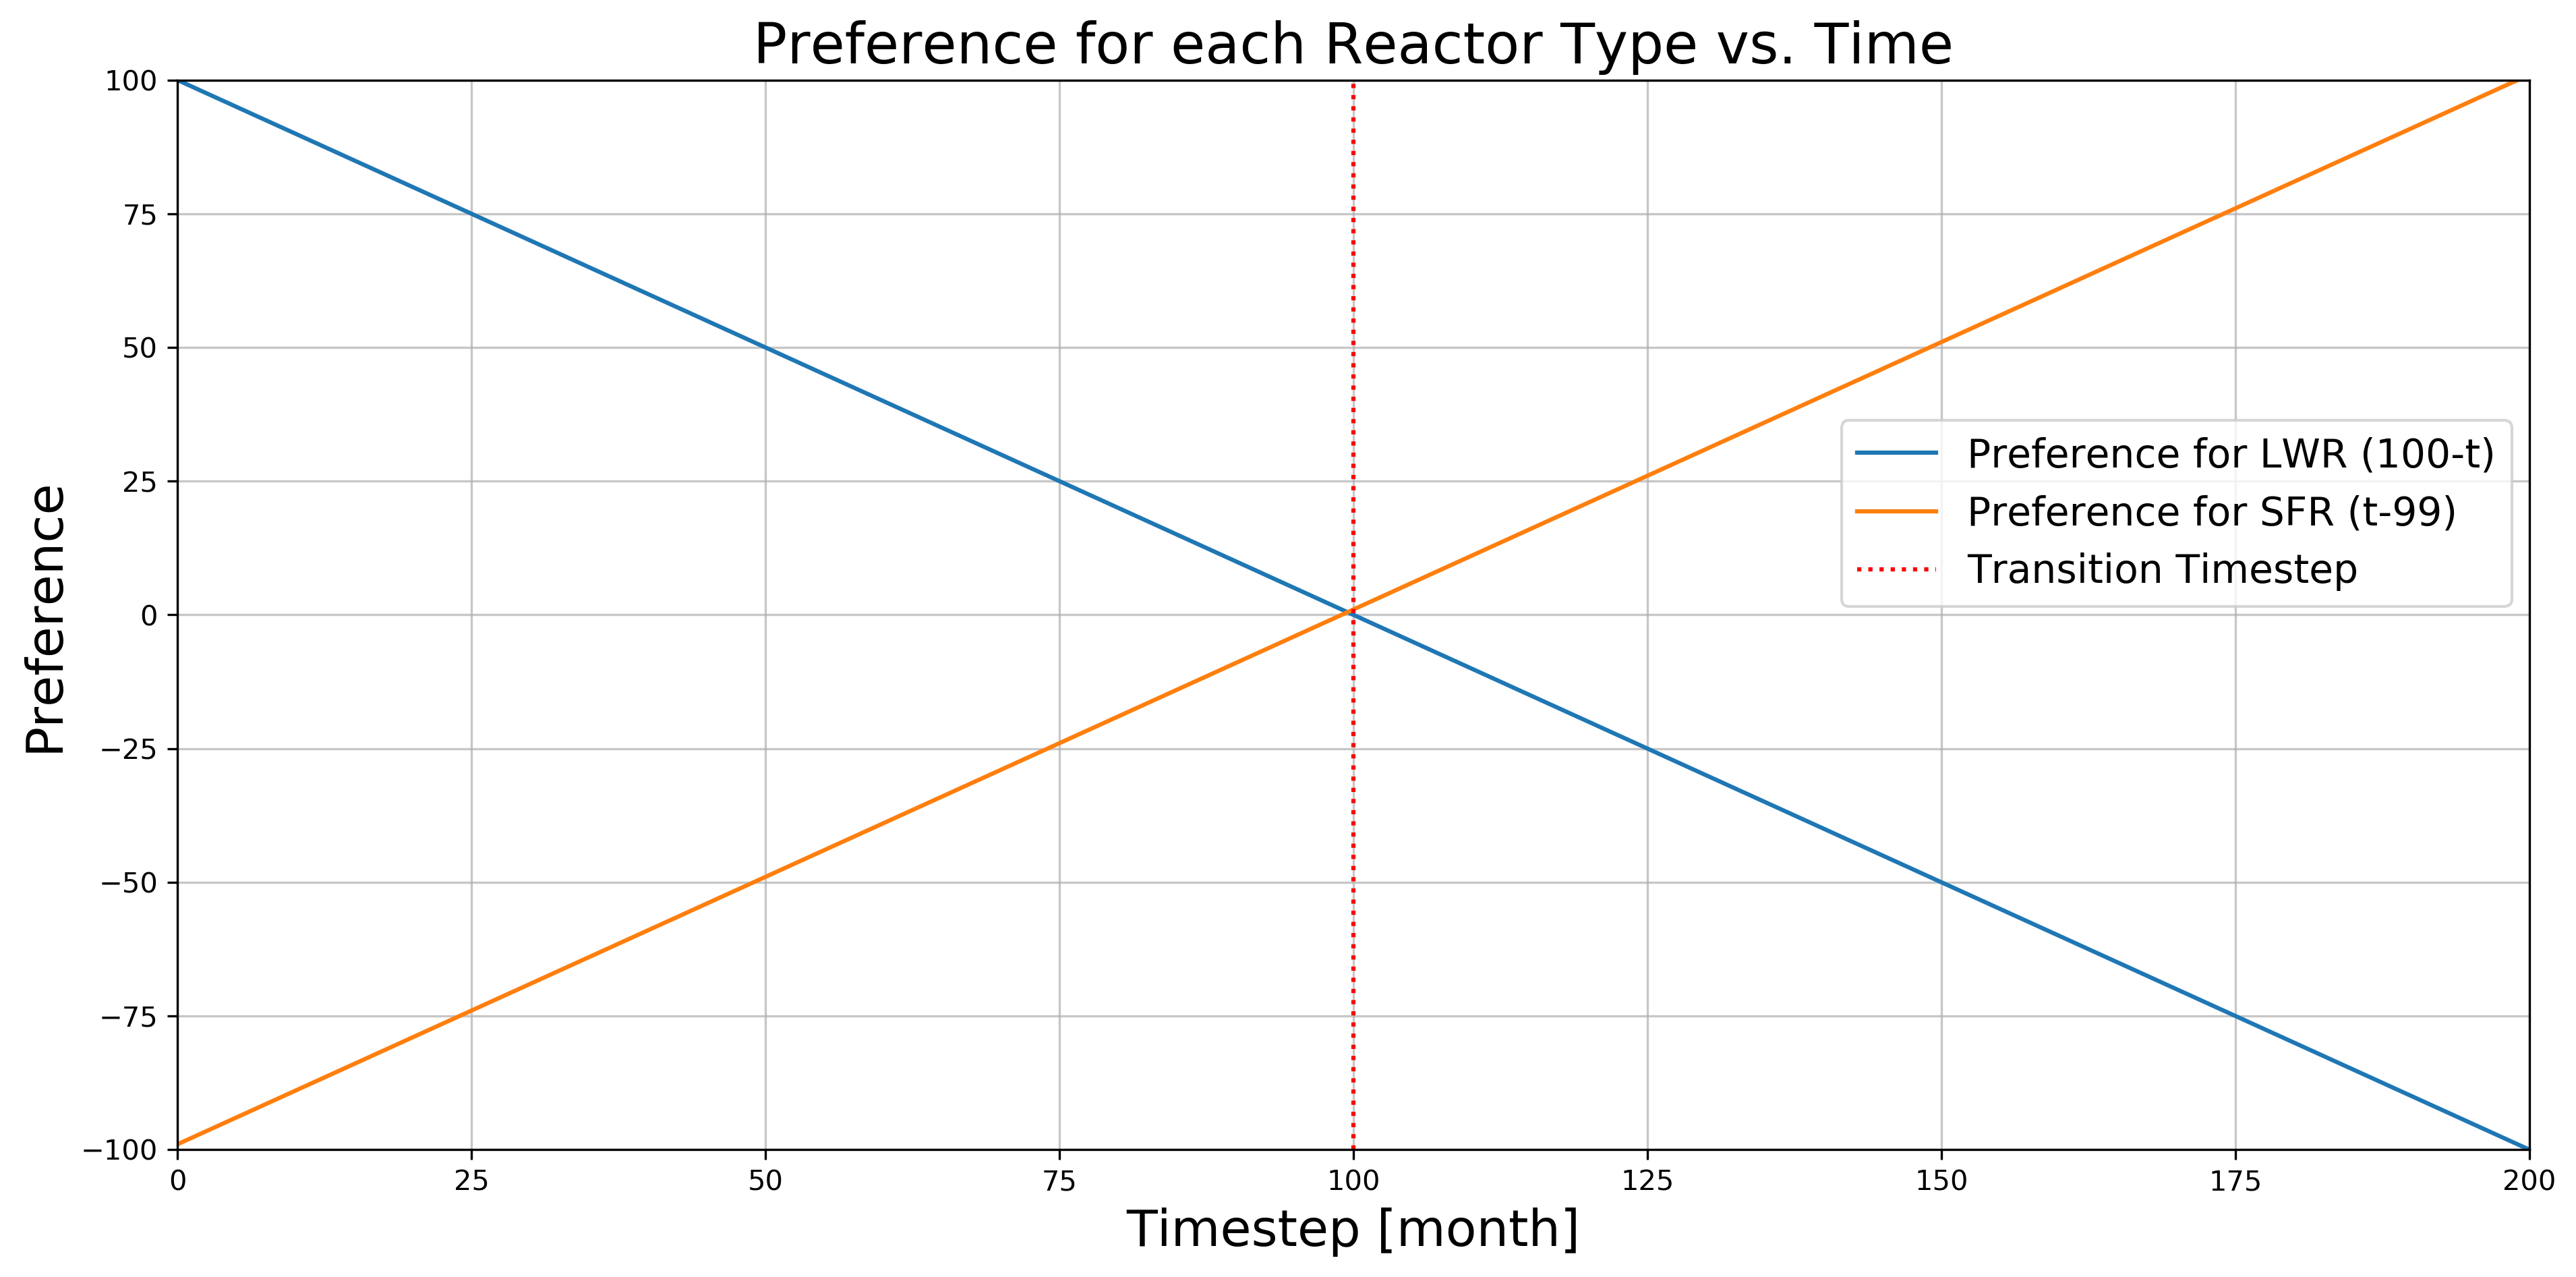
\includegraphics[width=\linewidth]{./figures/prefplot}
	\end{center}	
		\caption{\deploy has a $100-t$ preference for LWRs and a $t-99$ preference for SFRs.
		When there is a power undersupply, \deploy will deploy the reactor that has a
		larger preference at that time step.}
	\label{fig:prefplot}
\end{figure}

The user also has the option to specify percentage-share for facilities 
that provide the same commodity. 
For example, if there are two reactor types, \gls{MOX} LWRs and SFRs, in a simulation,
the user can make use of percentage-share specifications to determine the 
percentage of power supplied by each reactor.   
When MOX LWR has a share of $s\%$ and 
\gls{SFR} has a share of $(100-s)\%$, 
MOX LWR deployment constrains to $s\%$ of total power demand 
and SFR deployment constrains to $(100-s)\%$ of total power demand.  

The transition year is selected by customizing facility 
preferences to prefer advanced reactors at that year.
The fleet-share percentage determines the
share of each type of reactor to transition to. 
Figure \ref{fig:deployflow} shows the logical flow of
which facility \deploy deploys when there are multiple facilities 
offering the same commodity. 

\begin{figure}[]
	\centering
	\resizebox{0.9\textwidth} {0.8\height}{
    \begin{tikzpicture}[node distance=3cm]
    \tikzstyle{every node}=[font=\large]
    \node (fs)[olblock]{\textbf{Are there fleet share constraints?}};
    \node (fsyes) [bbmlock, below of=fs, xshift = -3.5cm] {\textbf{Deploy facilities to meet fleet share $\%$}};
    \node (pref) [olblock, right of=fsyes, xshift = 3.5cm]{\textbf{Are there facility \\ preferences?}};
    \node (prefyes) [bbmmlock, below of=pref, xshift = -3cm] {\textbf{Deploy facilities in preference order to meet their fleet share \%}};
    \node (prefno) [bbmlock, right of=prefyes, xshift = 3cm, yshift=-0.05cm] {\textbf{Deploy facilities to minimize total no. of facilities and minimize oversupply.}};
	\draw [arrow] (fs) -- node[anchor=east] {yes} (fsyes);
    \draw [arrow] (fs) -- node[anchor=east] {no} (pref);
    \draw [arrow] (pref) -- node[anchor=east] {yes} (prefyes);
    \draw [arrow] (pref) -- node[anchor=east] {no} (prefno);
	\end{tikzpicture}}
	
    \caption{Logical flow of how \deploy 
	selects which facility to deploy when there are multiple facilities 
	offering the same commodity.}
	\label{fig:deployflow}
\end{figure}

\subsection{Prediction Methods}
\label{sec:pm}
\deploy records supply and demand at each time step for all 
commodities. Time-series data informs \deploy's time series 
forecasting methods which predict future supply and demand for each 
commodity.  
The time series forecasting methods investigated include non-optimizing, 
deterministic-optimizing, and stochastic-optimizing methods. 
Non-optimizing methods are techniques that harness 
simple moving average and autoregression concepts which use 
historical data to infer future supply and demand values. 
Deterministic-optimizing and stochastic-optimizing 
methods are techniques 
that use an assortment of more sophisticated time series forecasting 
concepts to predict future supply and demand values. 
Deterministic-optimizing methods give deterministic solutions,
while stochastic-optimizing methods give stochastic solutions. 

Depending on the scenario in question, each forecasting method 
offers distinct benefits and disadvantages.
The various methods are compared for each type of simulation 
to determine the most effective prediction method for 
a given scenario. 
The following sections describe the prediction methods. 

\subsubsection{Non-Optimizing Methods}
Non-optimizing methods include: Moving Average (\texttt{MA}), 
Autoregressive Moving Average (\texttt{ARMA}), and 
Autoregressive Heteroskedasticity (\texttt{ARCH}). 
The \texttt{MA} method calculates the average of 
a user-defined number of previous entries in a commodity's 
time series and returns it as the predicted value 
(equation \ref{eq:ma}).

\begin{align}
	\label{eq:ma}
	Predicted\ Value &= \frac{\sum_{n=1}^N V_n}{n}
	\intertext{where:}
	V_n &= \mbox{Time series value} \nonumber\\
	N &= \mbox{length of timeseries} \nonumber\\
\end{align}

The \texttt{ARMA} method combines moving average and
autoregressive models (equation \ref{eq:arma}).
The first term is a constant, second term is 
white noise, the third term is the autoregressive
model, and the fourth term is the moving average
model.
The \texttt{ARMA} method is more accurate than the 
\texttt{MA} method 
because of the inclusion of the autoregressive term: 
\begin{align}
	\label{eq:arma}
	X_t &= c + \epsilon_t + 
	\sum_{i=1}^p\varphi_i X_{t-i} +	
	\sum_{i=1}^q\theta_i\epsilon_{t-i}.
	\intertext{where:}
    c &= \mbox{a constant} \nonumber\\
    \epsilon_t &= \mbox{error terms (white noise)} \nonumber\\
    \varphi &= \mbox{the autoregressive model’s parameters} \nonumber\\
    \theta &= \mbox{the moving average model’s parameters} \nonumber \\
    p &= \mbox{order of the autoregressive polynomial} \nonumber \\
    q &= \mbox{order of the moving average polynomial} \nonumber
\end{align}

The \texttt{ARCH} method models time series data by describing the 
variance of the current 
error term as a function of the sizes of the previous time periods' 
error terms \cite{engle_autoregressive_1982}. 
This allows the method to support changes in the time dependent volatility, 
such as increasing and decreasing volatility in the same series
\cite{engle_autoregressive_1982}.
The \texttt{ARCH} method is
better than the \texttt{ARMA} method for volatile 
time-series data \cite{flanagan_methods_2019}. 
The StatsModels \cite{seabold_statsmodels:_2010}
Python package is used to implement \texttt{ARMA} and 
\texttt{ARCH} methods in \deploy. 

\subsubsection{Deterministic-Optimizing Methods}
Deterministic methods include
Fast Fourier Transform (\texttt{FFT}), 
Polynomial Fit (\texttt{POLY}), 
Exponential Smoothing (\texttt{EXP-SMOOTHING}), 
and Triple Exponential Smoothing (\texttt{HOLT-WINTERS}). 
The \texttt{FFT} method uses the fast fourier transform
algorithm to map a time series into the frequency domain. 
The algorithm returns complex numbers from which frequency, 
amplitude, and phase is extracted. 
Future demand and supply values are predicted by summing 
the significant components, then using the inverse 
fourier transform method to return it into a usable form. 
The discrete fourier transform (DFT) transforms a sequence of 
N complex numbers ($X_k$) into another sequence of complex numbers
($x_n$) \cite{rao_fast_2011}:
\begin{align}
	\label{eq:fft}
	X_k &= \sum_{n=0}^{N-1}x_n e^{-i2\pi kn/N}.
    \intertext{where:}
    X &= \mbox{sequence of complex numbers} \nonumber \\
    k &= 0,...,N-1 \nonumber\\
    N &= \mbox{No. of complex numbers} \nonumber\\
    x &= \mbox{sequence of complex numbers} \nonumber \\
    n &= 0,...,N-1 \nonumber
\end{align}

This method is implemented in \deploy using the 
SciPy \cite{jones_scipy:_2016} Python package. 

The \texttt{POLY} method fits the time series data 
with a user-defined $n^{th}$ degree polynomial and uses 
the fitted trend-line to determine future demand and 
supply values: 

\begin{align}
    Y_t &= \beta_0 + \sum_{n=1}^N \beta_n t^n + \varepsilon \\
    \intertext{where:}
    t &= \mbox{time index} \nonumber \\
    n &= \mbox{polynomial order} \nonumber \\
    \beta &= \mbox{fitted parameters} \nonumber 
\end{align}

This method was implemented in \deploy using the 
NumPy \cite{oliphant_guide_2006} Python package. 
The \texttt{EXP-SMOOTHING} and \texttt{HOLT-WINTERS} 
methods use a weighted average 
of time-series data with exponentially decaying weights 
for older time series values \cite{hyndman_forecasting:_2018}
to create a model to determine future demand and supply values. 
The \texttt{EXP-SMOOTHING} method excels in 
modeling univariate time series data without trend or seasonality
\cite{hyndman_forecasting:_2018}: 

\begin{align}
    \label{eq:expsm}
    y_{t+1} &= \alpha y_i + (1-\alpha)y_t. \\ 
    \intertext{where:}
    y &= \mbox{timeseries value} \nonumber \\
    \alpha &= \mbox{smoothing factor } (0 < \alpha < 1)
\end{align}

The \texttt{HOLT-WINTERS} method applies triple exponential 
smoothing, resulting in higher accuracy when 
modeling seasonal time series data 
\cite{sematech_engineering_2006}: 

\begin{align}
    F_{t+m} &= (S_t +mb_t)I_{t-L+m} \\
    S_t &= \alpha \frac{y_t}{I_{t-L}}+(1-\alpha)(S_{t-1}+b_{t-1}) \nonumber \\
    b_t &= \gamma(S_t-S_{t-1})+)(1-\gamma)b_{t-1} \nonumber \\
    I_t &= \beta \frac{y_t}{S_t} + (1-\beta)I_{t-L} \nonumber \\
    \intertext{where:}
    F &= \mbox{forecast at m periods ahead} \nonumber \\
    t &= \mbox{time period index} \nonumber \\
    S &= \mbox{smoothed observation} \nonumber \\
    y &= \mbox{the observation} \nonumber \\
    b &= \mbox{trend factor} \nonumber \\
    I &= \mbox{seasonal index} \nonumber \\
    \alpha, \beta, \gamma &= \mbox{constants} \nonumber
\end{align}

The StatsModels \cite{seabold_statsmodels:_2010}
Python package was used to implement the \texttt{EXP-SMOOTHING} 
and \texttt{HOLT-WINTERS} methods in \deploy. 

\subsection{Stochastic-Optimizing Methods}
We implemented one stochastic-optimizing method: step-wise 
seasonal method (\texttt{SW-SEASONAL}
The method was implemented in \deploy by the auto \gls{ARIMA} 
method in the pmdarima \cite{smith_pmdarima:_2017}
Python package. 
The \gls{ARIMA} model is a dependent time series that is 
modeled as a linear combination of its own past values 
and past values of an error series \cite{institute_sas_1985}: 

\begin{align}
    (1-B)^dY_t &= \mu + \frac{\theta(B)}{\phi(B)}a_t \\ 
    \intertext{where:}
    t &= \mbox{time index} \nonumber \\
    \mu &= \mbox{mean term} \nonumber \\
    B &= \mbox{backshift operator, such that } BX_t = X_{t-1} \nonumber \\
    \phi(B) &= \mbox{autoregressive operator} \nonumber \\
    \theta(B) &= \mbox{moving average operator} \nonumber \\
    a_t &= \mbox{random error} \nonumber 
\end{align}

